\documentclass{beamer}
\usepackage{graphicx}
\graphicspath{ {images/} }
\usepackage{textcomp}
\usepackage{animate}
\usepackage{subcaption}
\usepackage[super]{nth}

\usetheme{Madrid}
\setbeamertemplate{caption}[numbered]

\theoremstyle{definition}
\newtheorem{defn}{Definition}
\newtheorem{thrm}{Theorem}

\AtBeginSection[]
{
  \begin{frame}
    \frametitle{Agenda}
    \tableofcontents[currentsection]
  \end{frame}
}

\title[CZ4079 FYP Presentation] {CZ4079 Final Year Project}
\subtitle{A Machine Learning-Based Approach to \\
Time-Dependent Shortest Path Queries}
\author[Wei Yumou]
{Wei Yumou}
\institute[]{School of Computer Science and Engineering \\ Nanyang Technological University}
\date[\today]{}
\logo{
\includegraphics[height=1cm]{logo}}

\begin{document}
\frame{\titlepage}

\section{Introduction}

\begin{frame}
\frametitle{Introduction: Problem}
\begin{itemize}
	\item <2-> A \textbf{dynamic road network} $G=(V,E)$ with a time-dependent weight function $w : E,t \rightarrow \mathbb{R}$
	\item <3-> A \textbf{query} $Q(u,v,t)$ that asks for a shortest path from $u$ to $v$ departing at time moment $t$
\end{itemize}
\end{frame}

\begin{frame}
\frametitle{Introduction: General Approach}
\begin{itemize}
	\item <2-> Traditional \textbf{Bellman-Ford or Dijkstra's algorithm}	do not work with dynamic edge weights (``the curse of traditionality'')
	\item <3-> The new \textbf{machine learning-based approach} draws on collective wisdom of thousands of taxi drivers
	\item <4-> \textbf{Unsupervised learning} is employed to figure out the time-dependent edge costs
	\item <5-> A modified Dijkstra's algorithm calculates a shortest path on the fly
\end{itemize}
\end{frame}

\begin{frame}
\frametitle{Introduction: Challenges}
\begin{itemize}
	\item <2-> Arbitrary $u$ and $v$
	\item <3-> Sparse sample points
	\item <4-> Limited GPS accuracy
\end{itemize}

\begin{figure}
\centering
\visible<3->{
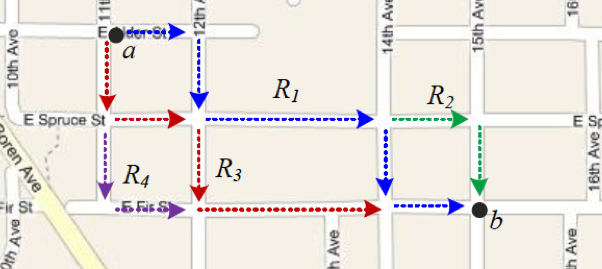
\includegraphics[width=0.4\textwidth, height = 3.5cm]{low_sample_rate}
}
\visible<4->{
    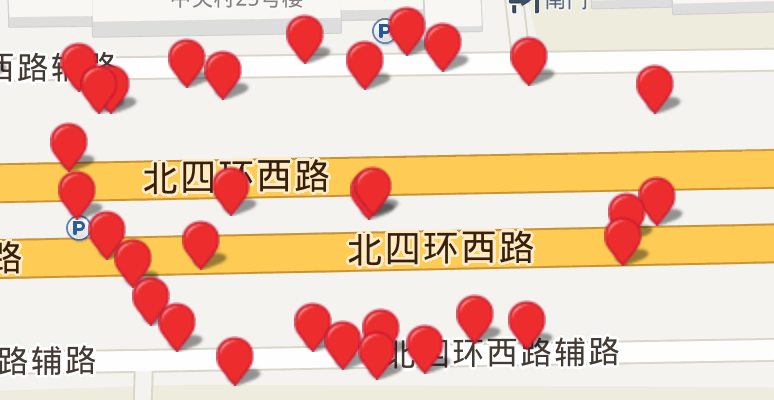
\includegraphics[width=0.4\textwidth, height = 3.5cm]{limited_accuracy}
     \caption{Examples of challenges} 
}
\end{figure}
\end{frame}

\section{Preliminary Processing}
\begin{frame}
\frametitle{Preliminary Processing: Data Description}

\begin{itemize}
	\item Is collected from Computational Sensing Lab at Tsinghua University
	\item Contains 83 million GPS records from 8,602 taxis in Beijing during May of 2009
\end{itemize}

\begin{table}[h!]
\centering
\resizebox*{0.5\textwidth}{!}{
\begin{tabular}{ | l | l | l | }
\hline
\textbf{Field} & \textbf{Explanation} \\ \hline
CUID & ID for each taxi \\ \hline
UNIX\_EPOCH & Unix timestamp \\ \hline
GPS\_LONG & Longitude in WGS-84\\ \hline
GPS\_LAT & Latitude in WGS-84 \\ \hline
HEAD & Heading direction \\ \hline
SPEED & Instantaneous speed (m/s)\\ \hline
OCCUPIED & Hired (1) or not (0) \\ \hline
\end{tabular}
}
\caption{A summary of the seven original fields}\label{Ta:orig_field}
\end{table}
\end{frame}

\begin{frame}
\frametitle{Preliminary Processing: Reverse Geocoding}
\begin{itemize}
	\item <2-> GPS coordinate translation: 1.34\textdegree N, 103.68\textdegree E~\textrightarrow~SCSE, NTU
	\item <3-> China GPS shift problem: WGS84 v.s. BD09
	\item <4-> Solution: WGS84~$\xrightarrow{Baidu\ API}$~BD09~$\xrightarrow{Baidu\ API}$~Street
\end{itemize}
\visible<3->{
\begin{figure}[h!]
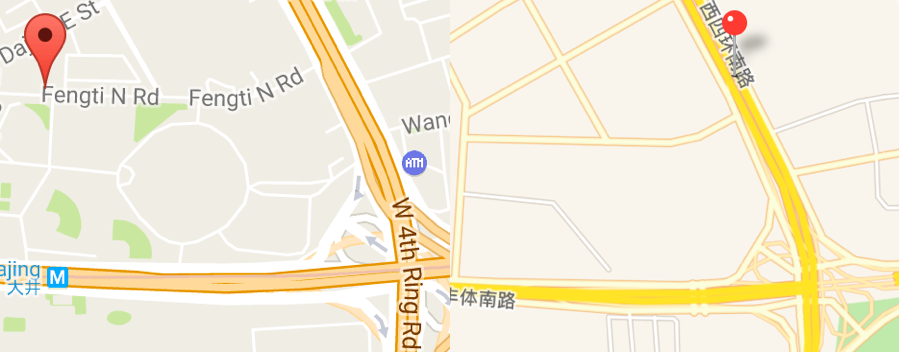
\includegraphics[scale=0.5]{gps_shift}
\centering
\caption{An example of China GPS shift problem}\label{Fig:gps_shift}
\end{figure}}
\end{frame}

\begin{frame}
\frametitle{Preliminary Processing: Outlier Detection}

\begin{figure}[h!]
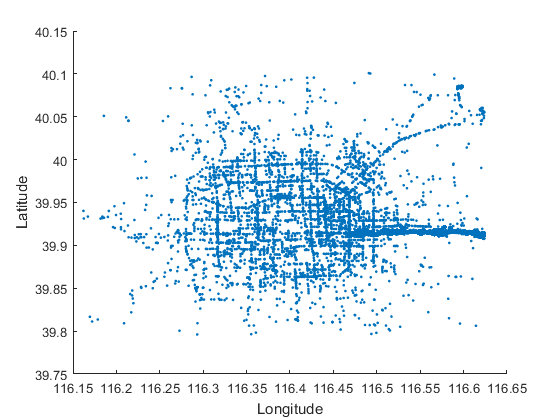
\includegraphics[scale=0.58]{outlier}
\centering
\caption{An example of outliers}\label{Fig:outlier}
\end{figure}

\end{frame}


\begin{frame}
\frametitle{Preliminary Processing: Outlier Detection}

\begin{thrm}[\emph{Majority Clustering Theorem}]\label{Theorem: majority_clustering}
If a \textbf{reasonable reverse geocoder} is used to reverse-geocode a set of GPS data points which are mapped to a particular street \emph{in reality}, then, when plotted on a 2-D plane, majority (more than 50\%) of the points must be clustered together to form a rough shape that is similar to the shape of the street that they are supposed to be mapped to. 
\end{thrm}

\visible <2->{
Two-step procedure:

Outlier Detection = Outlier Identification + Outlier Removal
}

\end{frame}

\begin{frame}
\frametitle{Preliminary Processing: Outlier Detection}
\textbf{Outlier Identification}: Clustering
\begin{itemize}
	\item <2-> Sample point concentration \textrightarrow~cluster concentration
	\item <3-> Top $k\%$ ($k = 50$) largest clusters as groups of correct sample points
	\item <4-> 10 \texttimes~10 self-organising feature maps implementation
\end{itemize}

\visible <5->{
\textbf{Outlier Removal}: Distance Threshold $d_{max}$
}
\begin{itemize}
	\item <6-> Assign sample points to legal centroids no farther than $d_{max}$
	\item <7-> Remove all ``orphan'' sample points
	\item <8-> Use real physical distance on the Earth
	\item <9-> Set $d_{max}$ = 30m or 50m
\end{itemize}

\end{frame}

\begin{frame}
\frametitle{Preliminary Processing: Outlier Detection}

\begin{figure}[h!]
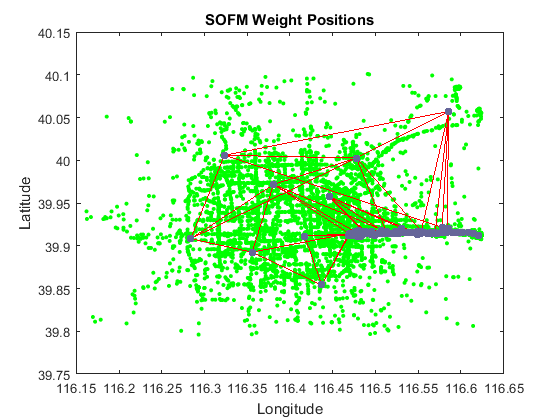
\includegraphics[scale = 0.48]{sofm_weights} 
\caption{A plot of neuron positions after training}
\label{Fig:sofm_weights}
\end{figure}
\end{frame}

\begin{frame}
\frametitle{Preliminary Processing: Outlier Detection}

\begin{figure}[h!]
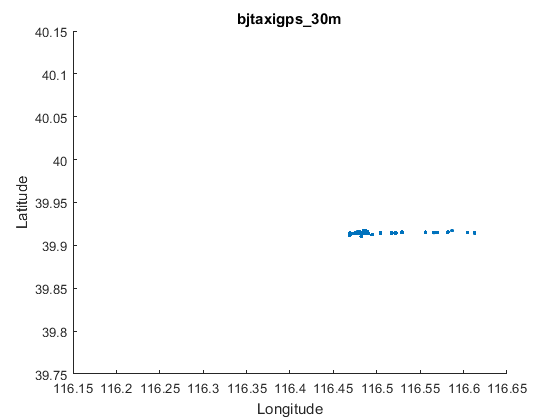
\includegraphics[width = 0.5\linewidth]{bjtaxigps_30m} 
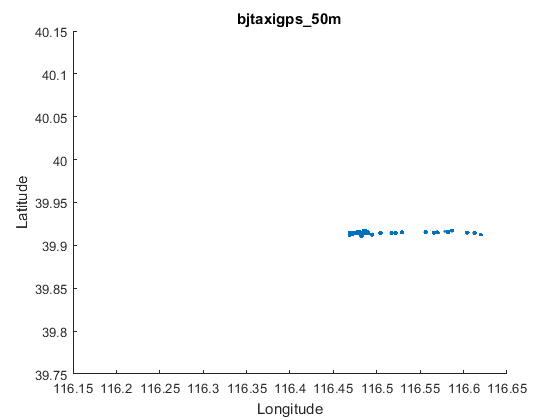
\includegraphics[width = 0.5\linewidth]{bjtaxigps_50m} 
\caption{A plot of sample points after outlier removal}\label{Fig:after_removal}
\end{figure}
\end{frame}

\section{Landmark Graph}

\begin{frame}
\frametitle{Landmark Graph: Basic Ideas}

\begin{defn}[\emph{Landmark}]\label{Def:ldmk}
A landmark is a road segment that is frequently traversed by taxi drivers according to the taxi GPS trajectory database. 
\end{defn}
\visible<2->{
Rationale
}
\begin{itemize}
	\item <2-> Sample points too sparse to model every street accurately
	\item <3-> Landmarks resemble common human thinking
\end{itemize}

\visible<4->{
Step to build landmark graph
}
\begin{itemize}
	\item <4-> Separate sample points into \textbf{trip}s
	\item <5-> Count occurrences of each street
	\item <6-> Find connections between two landmarks
\end{itemize}

\end{frame}

\begin{frame}
\frametitle{Landmark Graph: Trip Identification}
\begin{table}[h]
\centering
\resizebox{\columnwidth}{!}{
\begin{tabular}{ | l | l | l | l | l | l | l | l | l | l | l | l | l | }
\hline
\textbf{CUID} & \textbf{UTC} & \textbf{GPS\_LONG} & \textbf{GPS\_LAT} & \textbf{OCCUPIED} & \textbf{TRIP\_ID} \\\hline
1	&	1/5/2009 0:02:00	&	116.39616	&	39.81294	&	0	&	4552265\\ \hline
1	&	1/5/2009 0:04:00	&	116.39575	&	39.82296	&	0	&	4552265\\ \hline
1	&	1/5/2009 0:07:00	&	116.39567	&	39.82774	&	0	&	4552265\\ \hline
1	&	1/5/2009 17:08:00	&	116.30142	&	39.98105	&	1	&	1\\ \hline
1	&	1/5/2009 17:10:00	&	116.29514	&	39.98419	&	1	&	1\\ \hline
1	&	1/5/2009 17:11:00	&	116.28959	&	39.98289	&	1	&	1\\ \hline
1	&	1/5/2009 17:12:00	&	116.28087	&	39.97552	&	1	&	1\\ \hline
1	&	1/5/2009 17:16:00	&	116.26813	&	39.93537	&	1	&	1\\ \hline
1	&	1/5/2009 18:11:00	&	116.36537	&	39.95019	&	0	&	4552271\\ \hline
1	&	1/5/2009 18:12:00	&	116.36546	&	39.94886	&	0	&	4552271\\ \hline
1	&	1/5/2009 18:13:00	&	116.35927	&	39.94528	&	0	&	4552271\\ \hline
\end{tabular}}
\caption{An example of trip identification}\label{Ta:trip_identification}
\end{table}
\end{frame}

\begin{frame}
\frametitle{Landmark Graph: Frequency Counting}
\begin{table}[h!]
\centering
\resizebox{\columnwidth}{!}{
\begin{tabular}{ | l | l | l | l | l | l | l | l | l | l | l | l | l | }
\hline
\textbf{CUID} & \textbf{UTC} & \textbf{GPS\_LONG} & \textbf{GPS\_LAT} & \textbf{Street} & \textbf{TRIP\_ID} \\\hline
1	&	1/5/2009 0:02:00	&	116.39616	&	39.81294	&	A	&	4552265\\ \hline
1	&	1/5/2009 0:04:00	&	116.39575	&	39.82296	&	A	&	4552265\\ \hline
1	&	1/5/2009 0:07:00	&	116.39567	&	39.82774	&	B	&	4552265\\ \hline
1	&	1/5/2009 17:08:00	&	116.30142	&	39.98105	&	C	&	1\\ \hline
1	&	1/5/2009 17:10:00	&	116.29514	&	39.98419	&	C	&	1\\ \hline
1	&	1/5/2009 17:11:00	&	116.28959	&	39.98289	&	C	&	1\\ \hline
1	&	1/5/2009 17:12:00	&	116.28087	&	39.97552	&	A	&	1\\ \hline
1	&	1/5/2009 17:16:00	&	116.26813	&	39.93537	&	A	&	1\\ \hline
1	&	1/5/2009 18:11:00	&	116.36537	&	39.95019	&	B	&	4552271\\ \hline
1	&	1/5/2009 18:12:00	&	116.36546	&	39.94886	&	C	&	4552271\\ \hline
1	&	1/5/2009 18:13:00	&	116.35927	&	39.94528	&	C	&	4552271\\ \hline
\end{tabular}}
\caption{An illustration of frequency counting}\label{Ta:frequency_count}
\end{table}
\end{frame}

\begin{frame}
\frametitle{Landmark Graph: Construction}
For each trip
\begin{itemize}
	\item Select a landmark $j$
	\item Record intermediate streets while searching for the next landmark $k$
	\item Repeat the process starting from $k$ until all streets are examined
\end{itemize}
\end{frame}

\section{Travel Time Estimation}
\begin{frame}
\frametitle{Travel Time Estimation: Basic Ideas}

\begin{defn}[\emph{Significant Edge}]
A significant edge in a landmark graph $G=(V,E)$ is an edge $e \in E$ that has a support at least $m$, where $m$ is a parameter specified in advance.
\end{defn}
\begin{itemize}
	\item <2-> Build a \textbf{predictive model} for travel time of each significant edge
	\item <3-> Separate weekday's travel time from weekend's	
	\item <4-> Evaluate results against Baidu's estimates
\end{itemize}
\end{frame}

\begin{frame}
\frametitle{Travel Time Estimation: Underlying Distribution}
\begin{figure}[h!]
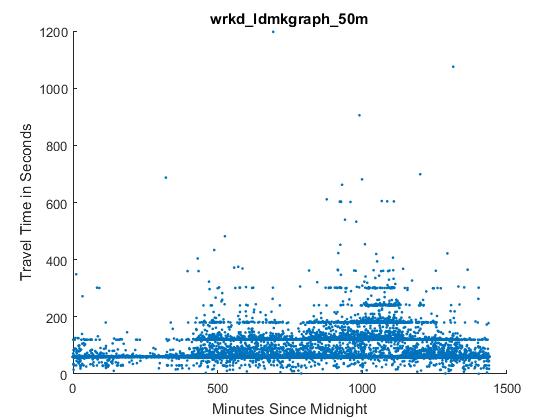
\includegraphics[scale=0.5]{trvltime_scatter}
\centering
\caption{An example of travel time patterns}\label{Fig:wrkd_50m_trvltime}
\end{figure}
\end{frame}

\begin{frame}
\frametitle{Travel Time Estimation: Underlying Distribution}
Possible Explanations
\begin{itemize}
	\item <1-> Drivers choose different routes to travel between the two landmarks
	\item <2-> Drivers have different driving skills, preferences and behaviours
	\item <3-> The GPS devices report locations \textbf{periodically}, therefore, durations like 60 seconds or 120 seconds are very common
\end{itemize}
\end{frame}

\begin{frame}
\frametitle{Travel Time Estimation: Clustering}
\begin{figure}[h!]
\centering
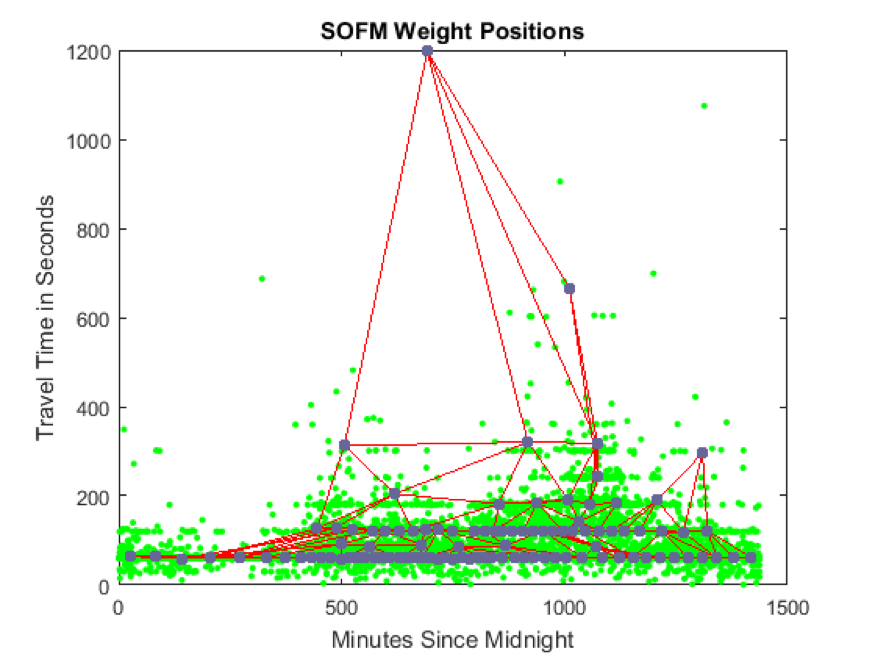
\includegraphics[scale = 0.4]{trvltime_clus}
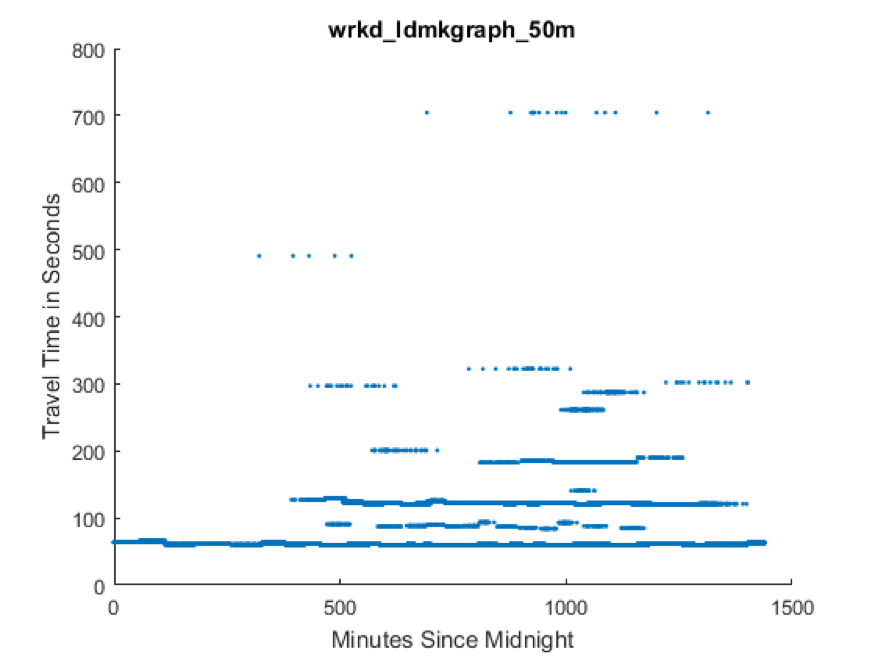
\includegraphics[scale = 0.4]{trvltime_neurons}
\caption{An illustration of travel time clustering} 
\end{figure}
\end{frame}

\begin{frame}
\frametitle{Travel Time Estimation: Distribution Fit}
\begin{figure}[h!]
\centering
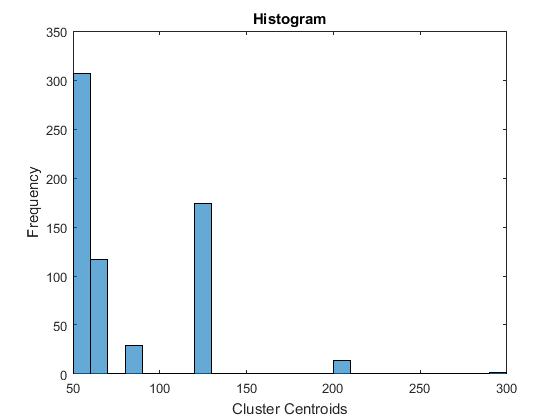
\includegraphics[scale = 0.4]{clus_histo}
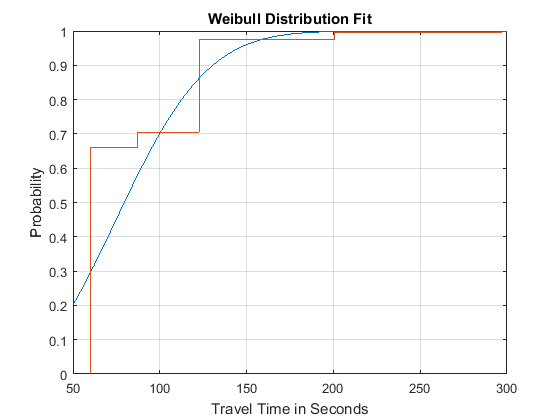
\includegraphics[scale = 0.4]{weibull_fit}
\caption{An illustration of fitting distribution} 
\end{figure}
\end{frame}

\begin{frame}
\frametitle{Travel Time Estimation: Implementation}
\begin{defn}[\emph{Optimism Index}]\label{Def:opti_index}
An optimism index indicates how optimistic a driver feels about his or her driving skills. A driver with an optimism index of $p\%$ usually drives faster than $(1 - p)\%$ drivers under similar road conditions.
\end{defn}
\begin{itemize}
	\item <1-> Calculate and store $\alpha$ and $\beta$ for each 30-minute window
	\item <2-> Use optimism index $p$ to find out travel time
\end{itemize}
\end{frame}

\begin{frame}
\frametitle{Travel Time Estimation: Evaluation}
\begin{itemize}
	\item <2-> Select the most significant 150 edges (pairs of landmarks)
	\item <3-> Sample 20\% of trips passing through each pair randomly
	\item <4-> Calculate travel time of each trip with optimism index $p = 0.5$
	\item <5-> Use Baidu Maps' API to give real-time estimates
	\item <6-> Compare Baidu's estimates with the \textbf{median} travel time 
\end{itemize}
\visible <7->{
\begin{table}[h!]
\centering
\resizebox{\textwidth}{!}{
\begin{tabular}{ | c | c | c | c |}
\hline
\textbf{Landmark Graph} & \textbf{RMSE} & \textbf{Mean Error Ratio} & \textbf{Mean No. of Samples Per Edge} \\ \hline
wrkd\_ldmkgraph\_50m & 78.84 & -0.009 & 1824.60 \\ \hline
wrkd\_ldmkgraph\_30m & 87.96 & -0.065 & 1507.56 \\ \hline
holi\_ldmkgraph\_50m & 87.39 & -0.16 & 832.96 \\ \hline
holi\_ldmkgraph\_30m & 76.41 & -0.14 & 681.89 \\ \hline
\end{tabular}}
\caption{A summary of evaluation results}\label{Ta:eval_res}
\end{table}
}
\end{frame}

\begin{frame}
\frametitle{Travel Time Estimation: Evaluation}
\begin{figure}[h!]
\centering
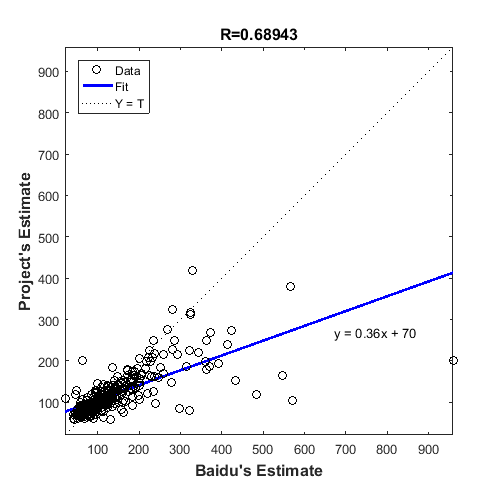
\includegraphics[scale = 0.4]{wrkd_50m_reg}
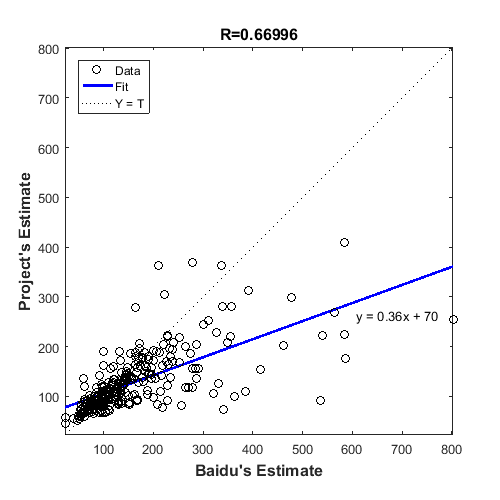
\includegraphics[scale = 0.4]{wrkd_30m_reg}
\caption{A plot of linear regression for weekday landmark graph}
\label{Fig:wrkd_reg}
\end{figure}
\end{frame}

\begin{frame}
\frametitle{Travel Time Estimation: Evaluation}

\begin{figure}[h!]
\centering
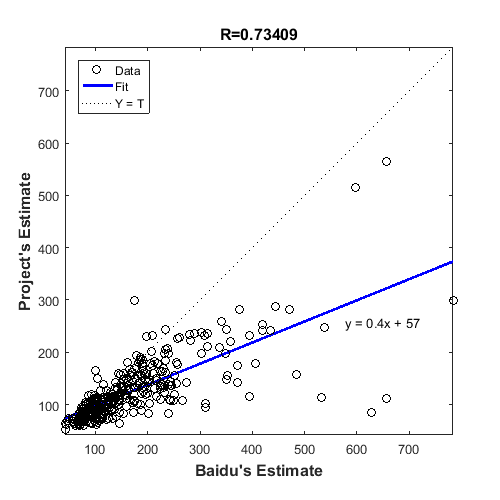
\includegraphics[scale = 0.4]{holi_50m_reg}
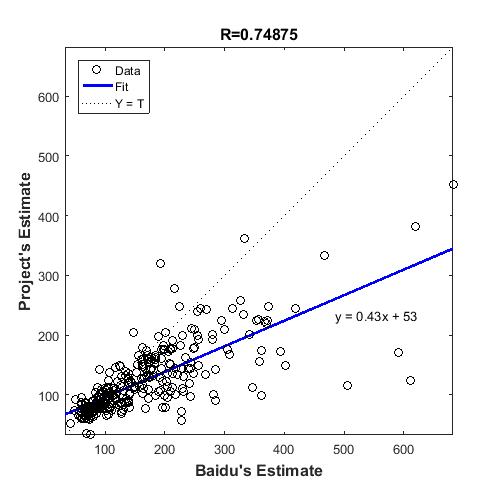
\includegraphics[scale = 0.4]{holi_30m_reg}
\caption{A plot of linear regression for weekend landmark graph}
\label{Fig:holi_reg}
\end{figure}
\end{frame}
%
%\begin{frame}
%\frametitle{Conclusion}
%\begin{itemize}
%	\item TrueSkill\texttrademark~algorithm can give a reasonable estimate of the ``true skill'' of a player (team) and calculate the wining probability of a future match
%	\item We selected three more features to give a better prediction
%\end{itemize}
%\end{frame}
%
%\begin{frame}
%\frametitle{Questions \& Answers}
%\begin{center}
%\huge Any questions?
%\end{center}
%\end{frame}

\end{document}